\section{Introduction}\label{sec:intro}




%background: image generation 
The field of image generation has recently experienced significant growth, driven by advancements from both academic and industrial researchers. Recent models, such as DALLE-3 and Stable Diffusion 3~\cite{sd3}, have elevated text-conditioned image generation to unprecedented levels. These models, requiring only simple textual instructions, demonstrate remarkable capability in generating high-quality images with intricate details. 
These approaches typically involve a classifier-free mechanism during the diffusion process to integrate conditions. For example, in the widely adopted Stable Diffusion, text prompts work as conditions of the diffusion network via cross-attention mechanisms to enable text-to-image translation.

Recent studies have also explored image generation conditioned on multi-modal prompts, which require simultaneous guidance from multiple modalities. For example, IP-Adapter~\cite{ye2023ip} guides image generation by referring to both image prompts and textual instructions, through developed cross-attention modules. Similarly, FaceStudio~\cite{yan2023facestudio} adopted a hybrid guidance framework and could utilize stylized images, facial images, and textual prompts as conditions for personalized portrait generation.
Based on these techniques, a variety of interesting applications have emerged, such as subject-driven image generation~\cite{pan2023kosmos, li2024blip, purushwalkam2024bootpig}, personalized image generation~\cite{wang2024instantid, yan2023facestudio}, and artistic portrait creation~\cite{ye2023ip}.
However, previous works employ distinct strategies for multi-modal prompts, and the genetic architecture of general multi-modal guided image generation remains unknown.

One of the main challenges facing current design paradigms is how to balance various conditions. During the image generation process, when multiple conditions are used, current methods may tend to favor certain conditions over others. For instance, it is observed that IP-Adapter~\cite{ye2023ip}, which relies on text prompts and image features as conditions, may predominantly be influenced by the image features. 
This can be attributed to the inherent limitations within the model architectures of existing methods, which do not effectively manage the varying complexities associated with different conditions. When training a model on multi-modal prompts, it often learns to control just one condition effectively, neglecting more challenging ones. This results in a bias towards easier conditions. For example, if a network is trained with both an object image and its description as conditions, it might overly rely on the image to generate object appearance, failing to adequately learn from the description. This issue highlights the need for strategies in training that ensure balanced learning across all conditions to maintain the model's versatility and fairness.
Furthermore, the scarcity of multi-modal training datasets in specialized domains exacerbates the issue. Taking subject-driven image generation as an example, a series of models (Kosmos-g~\cite{pan2023kosmos}, BootPig~\cite{purushwalkam2024bootpig}, SSR-Encoder~\cite{zhang2023ssr}) uses cropped object images to serve both as conditions and as the ground truth, which is a common practice in this area. However, models trained on such datasets are limited to a simple copy-paste functionality and may ignore the textual conditions. The absence of suitable training datasets becomes increasingly problematic with an increasing number of conditions. The limitations of model architecture and the lack of appropriate training datasets make it difficult to achieve a balanced approach for image generation models with multiple conditions.



To address the challenge above, we aim to design a more flexible paradigm for multi-modal guidance, that could well balance multiple conditions. 
In this paper, we introduce EMMA. Our proposed EMMA is built upon the state-of-the-art text-conditioned diffusion model ELLA~\cite{hu2024ella}, which trains a transformer-like module, named Perceiver Resampler, to connect text embeddings from pre-trained text encoders and pre-trained diffusion models for better text-guided image generation.
ELLA can effectively utilize pre-trained text and diffusion knowledge to achieve SOTA results in dense prompt-based image generation without the need to adjust their raw parameters. 
ELLA has strong text-to-image generation ability, and our proposed EMMA could merge information from other modalities into text features for guidance. This is inspired by Flamingo~\cite{alayrac2022flamingo}, a multi-modal large language model aiming at multi-modal understanding. Flamingo employs a strategy where it encodes images and text separately and integrates image features into text features using cross-attention within various transformer layers in the large language model. In this way, Flamingo adopts text as the primary carrier of information and integrates information from other modalities into LLM precisely for multi-modal understanding. 
Similarly, leveraging the transformer structure used by ELLA, which extracts features from the LLM to inject into SD, we introduce information from other modalities in the intermediate layers of these transformers to facilitate multimodal guidance.


In detail, to control the image generation process by modalities beyond text, EMMA incorporates our proposed Assemblable Gated Perceiver Resampler (AGPR), which leverages cross-attention to inject information from additional modalities beyond texts. In our design, the AGPR blocks are strategically interleaved with the blocks of the Perceiver Resampler of ELLA. This arrangement ensures an effective integration of multi-modal information. 
During training, we freeze the raw modules of ELLA to maintain the control ability of text conditions. Finally, we get a series of models based on different conditions, such as text features combined with facial features, and text features combined with object-level image features. 

Notably, EMMA is inherently designed to handle multi-modal prompts as conditions, allowing for the straightforward combination of different multi-modal configurations. This is achieved by the gate mechanism in our AGPR, which could control the way of injecting information from other modalities into the textual features. This advantage enables diverse and complex inputs to be synthesized into a unified generation framework without the need for additional training.
For example, image features can be utilized to depict the main subject, while finer-grained facial features provide identity information. 

As EMMA does not necessitate modifications to the underlying diffusion model, i.e. the U-net model or DiT~\cite{chen2023pixart, dit} model, 
it is readily compatible with a multitude of existing works based on the Stable Diffusion framework. By directly replacing the condition modules with EMMA, a series of interesting applications could be produced with no need for further training, such as Portrait generation, Cartoon generation, and subject-driven video generation shown in Figure~\ref{fig:teaser}. 

\begin{figure}[t]
    \centering
    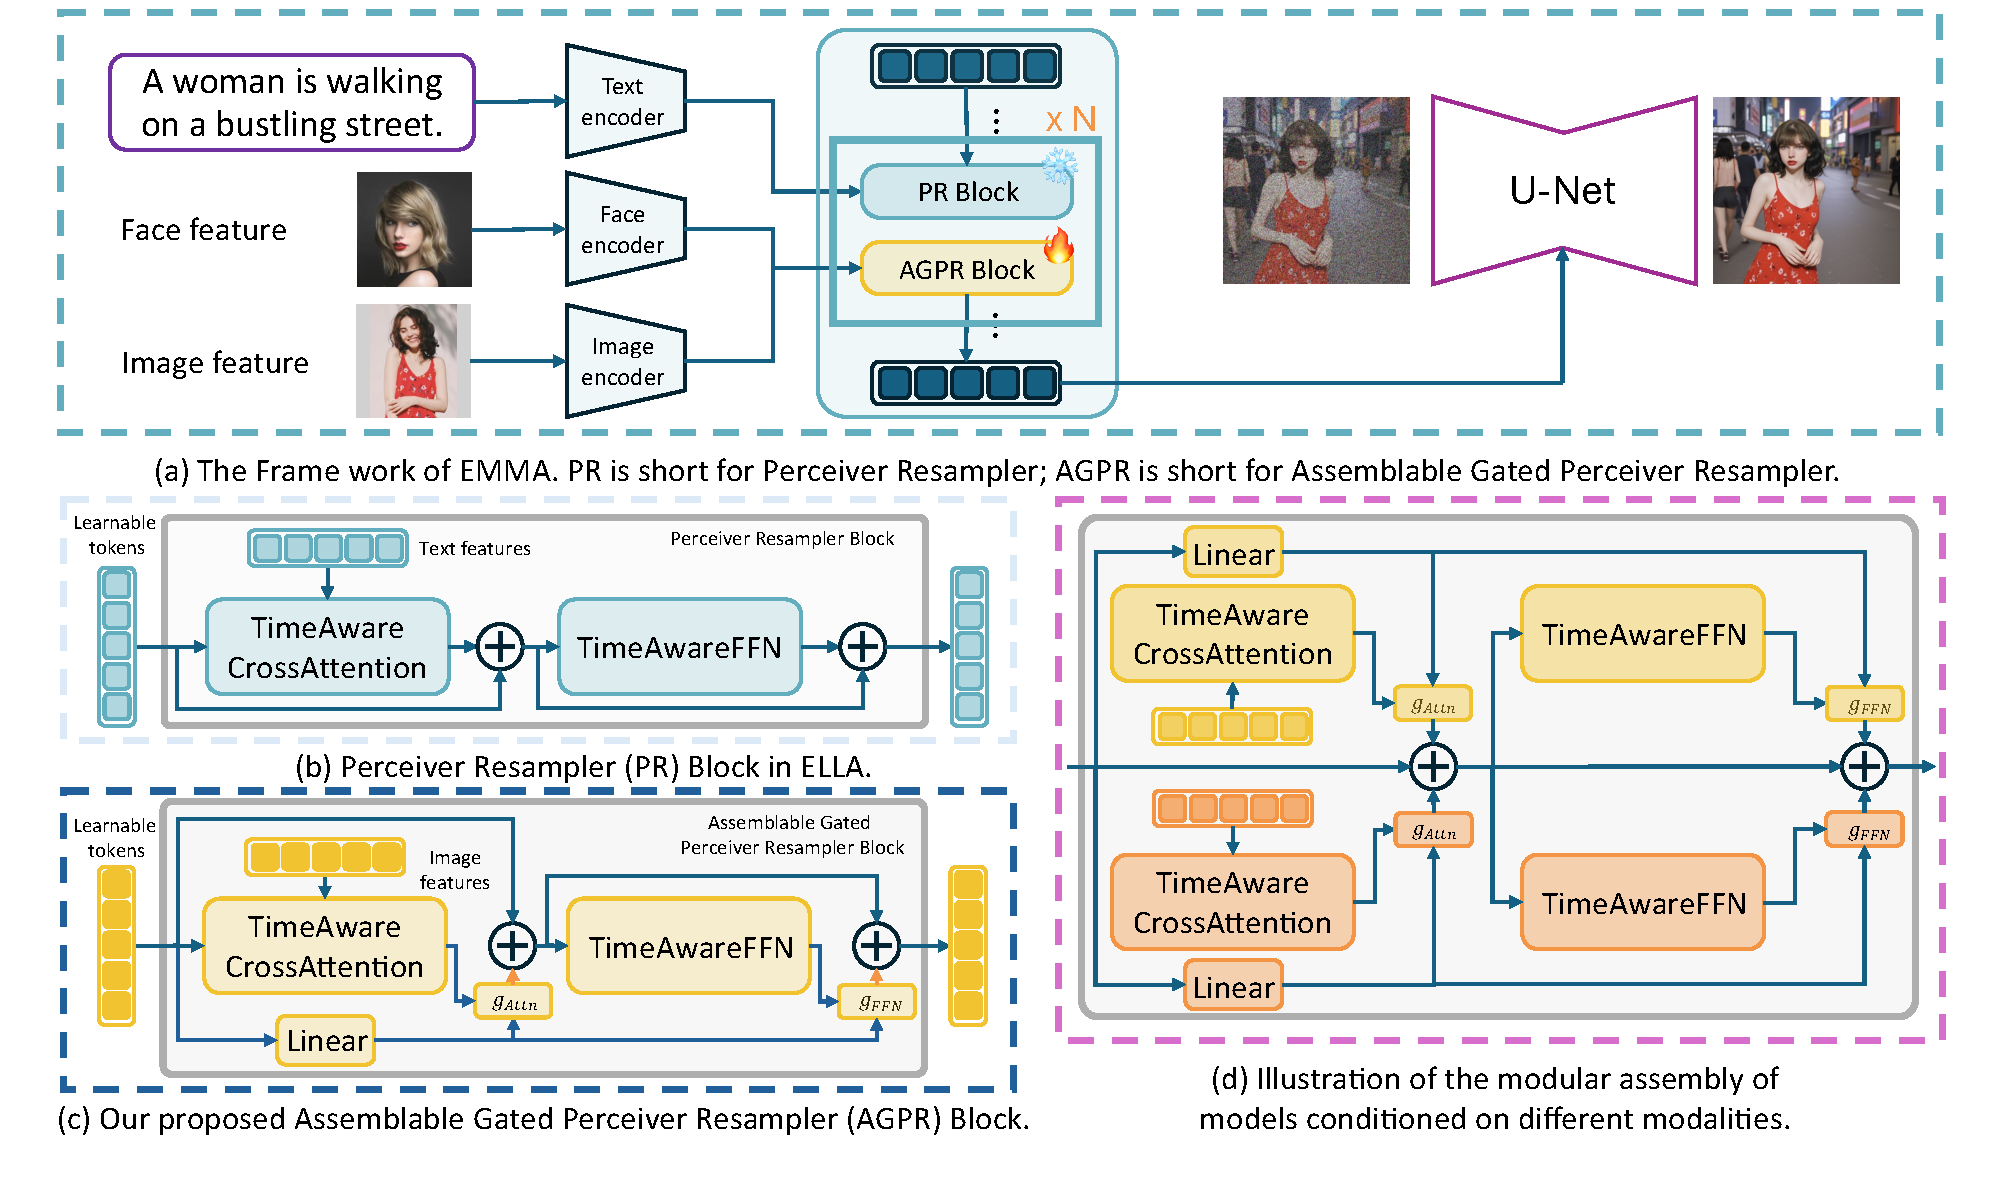
\includegraphics[width=0.95\textwidth]{images/methods.pdf}
    \caption{The model architecture of our proposed EMMA. (a) The framework of our EMMA. (b) The architecture of the Perceiver Resampler block proposed in ELLA~\cite{hu2024ella} (c) The architecture of our Assemblable Gated Perceiver Resampler block. The orange part is the novel part introduced in our AGPR block compared with the Perceiver Resampler block. (d) The pipeline of the composite process. }
    \label{fig:methods}
\end{figure}

Our key contributions are as follows:
\begin{enumerate}
    \item \textbf{Novel Integration Mechanism for Multi-modal prompts}: We introduce the EMMA, a pioneering approach that merges features of multi-modal prompts into the image generation process without compromising textual control. Our approach significantly enhances the flexibility and applicability of image generation by enabling the synergistic interaction of multiple modalities. This innovation allows for the creation of high-quality images that are responsive to a variety of input conditions.
    \item \textbf{Modular and Efficient Model Training}: Our framework facilitates the modular assembly of models conditioned on different modalities, streamlining the process and eliminating the need for retraining when new conditions are introduced. This efficient training procedure conserves resources and accelerates the model's adaptability to novel tasks.
    \item \textbf{Universal Compatibility and Adaptability}: EMMA works as a plug-and-play module without fine-tuning for a spectrum of existing and emerging models, including various image and video generation applications. Its compatibility with the Stable Diffusion framework and other models enhances its utility across diverse domains.
    \item \textbf{Robust Performance and Detail Preservation}: Through our experiments, we have confirmed the robustness of the EMMA model against various control signals, ensuring that it preserves both textual and visual details in the generated images. The model's architecture is designed to be scalable and flexible, accommodating a wide range of conditions and applications while maintaining high fidelity and quality.
\end{enumerate}